\documentclass[11pt,twocolumn]{article}
\raggedbottom

% --- Codificación y lenguaje ---
\usepackage[T1]{fontenc}
\usepackage[utf8]{inputenc}
\usepackage[spanish]{babel}

% --- Matemática y fuentes ---
\usepackage{amsmath, amsfonts, amssymb, amsthm}
\usepackage{derivative}

% --- Gráficos y tablas ---
\usepackage{graphicx}   % ya lo usas
\usepackage{animate}    % paquete para animaciones
\usepackage{caption}        % <-- primero caption
\usepackage{subcaption}     % <-- luego subcaption
\usepackage{booktabs}
\usepackage{ulem} % for \sout
\usepackage{siunitx}

% --- Varios útiles ---
\usepackage[margin=2cm]{geometry}
\setlength{\emergencystretch}{3em}
\usepackage{enumitem}
\usepackage{csquotes}
\usepackage{cuted}          % para elementos a dos columnas (opcional)
\usepackage{stackrel}
\usepackage{float}
\usepackage{placeins}
\usepackage{multirow}
% \usepackage{nameref}      % NO necesario: hyperref ya define \nameref
\usepackage[dvipsnames]{xcolor}
\usepackage{tikz}
\usetikzlibrary{calc}

% --- Bibliografía (BibTeX + apacite) ---
\usepackage[backend=biber,style=apa,language=spanish]{biblatex}
\addbibresource{references.bib}


% --- Hipervínculos (casi al final) ---
\usepackage[
  colorlinks=true,
  linkcolor=black, urlcolor=black, citecolor=black, filecolor=black,
  pdfborder={0 0 0}
]{hyperref}
% --- Colores para hipervínculos (citas en azul) ---
\hypersetup{
  colorlinks=true,
  linkcolor=black,      % refs, índice
  urlcolor=Blue,
  citecolor=Blue   % color del link de la cita
}

% --- Citas en azul mediante hyperref ---
% El color de las citas queda controlado por citecolor=Blue.

\begin{document}

\begin{tikzpicture}[remember picture,overlay]
  \node[anchor=north east, inner sep=0pt]
    at ($(current page.north east)+(-1.8cm,-1.2cm)$)
    {
\includegraphics[height=2.8cm]{UdeC_logo_azul.png}};
\end{tikzpicture}

\begin{strip}
\begin{center}
\vspace*{-5\baselineskip}
{\Large \textbf{Universidad de Concepción}}\\[-2pt]
\small Facultad de Ciencias Físicas y Matemáticas\\[-2pt]
\small \textit{Física VII Introducción a la Mecánica Cuántica (510322-1)}\\[4pt]

{\Large \bfseries Informe 1: Difracción de la Luz}\\
[2pt]
\small Profesor: Paulraj Manidurai\\[-2pt]
\small N. Ulloa C., J. Rosas S.\\[-2pt]
\small Concepción, Chile — 20 de octubre de 2025
\end{center}
\vspace{0.5\baselineskip}
\hrule
\vspace{0.8\baselineskip}

% ===========================
% 0. Abstract.
% ===========================

\begin{abstract}

Se caracterizó una red de difracción de transmisión de 600~líneas/mm y se determinó la longitud de onda de varias componentes visibles. A partir de las posiciones angulares de los máximos de difracción de primer orden, se obtuvieron longitudes de onda desde el rojo hasta el violeta, en buen acuerdo con los rangos conocidos del espectro visible, con incertidumbres del orden de decenas de nanómetros. Esto muestra que el montaje funciona como un espectrómetro sencillo.


\end{abstract}

\noindent\rule{\textwidth}{0.4pt}\par\vspace{0.3cm}
\end{strip}

% ===========================
% 1. Objetivos.
% ===========================

\section{Objetivo.}

\begin{itemize}
    \item Medir los ángulos de difracción $\theta$ asociados al primer máximo de interferencia ($m=1$) para distintas componentes de color de una fuente luminosa.
    \item Determinar las longitudes de onda $\lambda$ correspondientes a cada color, junto con su incertidumbre experimental.
    \item Evaluar la reproducibilidad de las mediciones repitiendo el montaje óptico y comparando ambos conjuntos de resultados.
    \item Discutir en qué medida la red de difracción puede utilizarse como analizador espectral para separar colores cercanos.
\end{itemize}

% ===========================
% 3. Marco teórico.
% ===========================
\section{Marco teórico.}

\subsection{Naturaleza ondulatoria de la luz}

La luz visible puede describirse como una onda electromagnética transversal que transporta energía y momento (véase la Figura~\ref{fig:onda_em}). En el régimen de óptica física, la luz se modela como campos eléctricos y magnéticos que oscilan en el tiempo y avanzan en el espacio como frentes de onda \cite{hecht_optics,young_freedman}. Fenómenos como la interferencia y la difracción no son correcciones pequeñas, sino manifestaciones directas de la superposición de frentes de onda coherentes: distintas porciones de una misma onda pueden reforzarse o anularse entre sí, generando máximos y mínimos de intensidad \cite{pedrotti_optics}.

Cuando una onda luminosa encuentra una abertura o un obstáculo de tamaño comparable a su longitud de onda $\lambda$, el frente de onda deja de propagarse estrictamente en línea recta y se “abre” angularmente: este fenómeno es la difracción. El efecto es especialmente marcado si la luz atraviesa no sólo una rendija, sino muchas rendijas igualmente espaciadas: una \textbf{red de difracción} \cite{hecht_optics,tipler_mosca}.

\begin{figure}
    \centering
    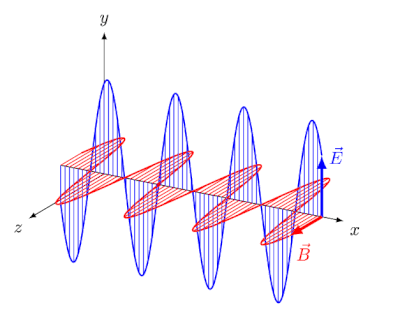
\includegraphics[width=1\linewidth]{figures/ondas-electromagneticas.png}
    \caption{
    Propagación de una onda electromagnética: el campo eléctrico $\vec E$
    y el campo magnético $\vec B$ oscilan en planos perpendiculares entre sí
    y a la dirección de propagación. La animación ilustra el carácter transversal
    de la luz visible.
    }
    \label{fig:onda_em}
\end{figure}

\subsection{Red de difracción como interferómetro multirendija}

Una red de difracción de transmisión es un conjunto de $N$ ranuras paralelas, regularmente espaciadas sobre un soporte transparente. Si llamamos $a$ al espaciamiento entre centros de ranuras adyacentes (el \emph{paso} de la red), entonces ``600 líneas/mm'' significa que en \SI{1}{mm} caben 600 periodos ranura+banda opaca, de modo que
\begin{equation*}
    a \approx \frac{1\ \text{mm}}{600}
    \approx 1{,}67\times 10^{-6}\ \text{m}.
\end{equation*}
Este parámetro geométrico $a$ fija la periodicidad espacial del sistema y determina en qué direcciones habrá interferencia constructiva \cite{hecht_optics,pedrotti_optics}.

Cada ranura actúa aproximadamente como una fuente secundaria coherente. Como todas las ranuras están iluminadas por el mismo haz incidente, las ondas emergentes mantienen fases bien definidas entre sí. La interferencia entre estas $N$ fuentes es análoga al experimento de doble rendija de Young, pero mucho más direccional: en ciertos ángulos todas las contribuciones suman en fase y la intensidad es máxima; en otros ángulos se cancelan \cite{young_freedman}.

\subsection{Condición de máximos de difracción}

Sea $\theta_m$ el ángulo entre la dirección de observación y el eje del haz incidente. La diferencia de camino óptico entre dos ranuras vecinas es
\begin{equation*}
    \Delta \;=\; a \,\sin\theta_m.
\end{equation*}
Si esa diferencia es un múltiplo entero de la longitud de onda $\lambda$, las ondas llegan en fase y la interferencia es constructiva. Esto lleva a la condición de máximos de difracción:
\begin{equation}
    a \,\sin\theta_m \;=\; m\,\lambda,
    \qquad m = 0, \pm1, \pm2, \ldots
    \label{eq:maximos}
\end{equation}
donde $m$ es el \emph{orden de difracción} \cite{hecht_optics,tipler_mosca}.  

El máximo $m=0$ corresponde al haz directo (sin desviación). Los máximos $|m|=1$ son las primeras franjas brillantes a ambos lados del haz central. Órdenes superiores ($|m|\ge 2$) suelen ser menos intensos, pero aparecen más separados angularmente \cite{pedrotti_optics}.

En este experimento sólo analizamos $m=1$ porque (i) es fácil de identificar respecto del máximo central, (ii) tiene intensidad suficiente para trabajarlo en laboratorio sin instrumentación especializada y (iii) evita confusiones entre órdenes distintos.

\begin{figure}[H]
    \centering
    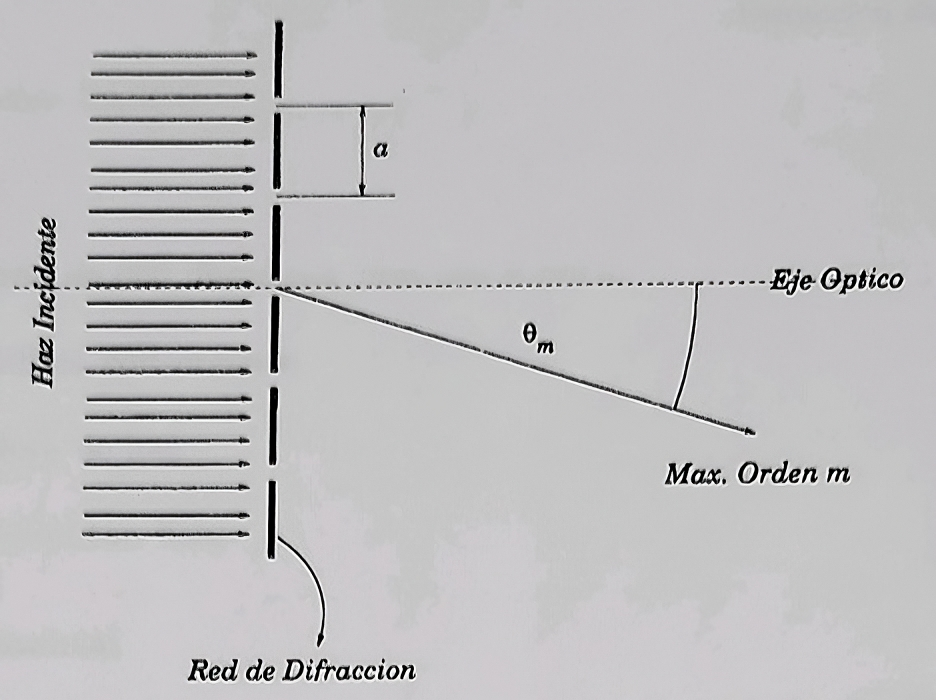
\includegraphics[width=1\linewidth]{figures/fig1.png}
    \caption{
    Difracción de la luz en una red de transmisión. 
    El haz incidente atraviesa las múltiples ranuras periódicas (paso $a$), 
    y la interferencia constructiva concentra luz en ángulos definidos $\theta_m$.
    Cada ángulo $\theta_m$ corresponde a un máximo de orden $m$ que satisface
    $a \sin\theta_m = m \lambda$.
    }
    \label{fig:principio_red}
\end{figure}

\subsection{Geometría experimental para medir \texorpdfstring{$\lambda$}{lambda}}

En el banco óptico, la red se fija en una montura y, a una distancia conocida $L$, se coloca una regla graduada. Observando a través de la red se ve que el máximo de primer orden ($m=1$) aparece desplazado lateralmente una distancia $x$ respecto del eje óptico (véase Figura~\ref{fig:geometria_medicion}).

Este desplazamiento define la geometría de un triángulo rectángulo:
\begin{equation}
    \tan\theta = \frac{x}{L}.
    \label{eq:tan-theta}
\end{equation}
De aquí,
\begin{align*}
    \theta = \arctan\!\left(\frac{x}{L}\right),\\[6pt]
    \sin\theta = \frac{x}{\sqrt{x^{2}+L^{2}}}.
\end{align*}

Sustituyendo esta última expresión en \eqref{eq:maximos} con $m=1$ se obtiene la relación experimental directa:
\begin{equation}
    \lambda
    \;=\;
    a \,\frac{x}{\sqrt{x^{2}+L^{2}}}
    \qquad (m=1).
    \label{eq:lambda-experimental}
\end{equation}
La ecuación \eqref{eq:lambda-experimental} vincula únicamente cantidades geométricas medibles ($x$ y $L$) con la longitud de onda física $\lambda$ del haz transmitido por la red. En este sentido, el montaje actúa como un \textit{espectrómetro elemental}: cada color (cada $\lambda$ distinta) produce un máximo en un ángulo distinto y, por tanto, en una posición $x$ distinta sobre la escala \cite{hecht_optics,tipler_mosca,young_freedman}.

\begin{figure}[H]
    \centering
    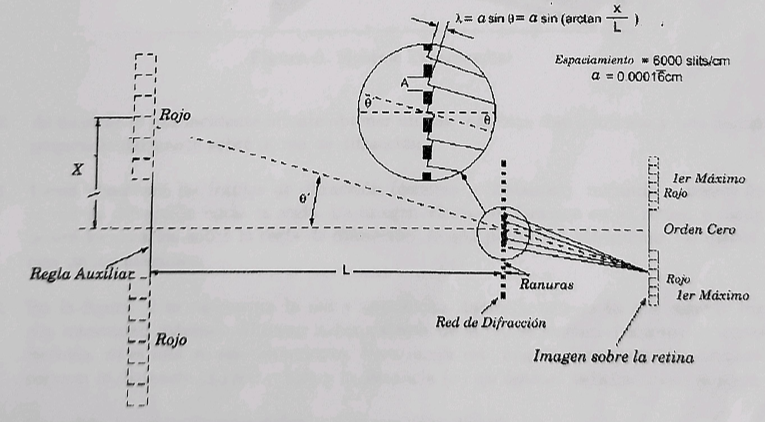
\includegraphics[width=\linewidth]{figures/fig2.png}
    \caption{
    Geometría de medición. 
    El máximo de primer orden ($m=1$) aparece desplazado una distancia $x$ en la regla,
    situada a una separación fija $L$ de la red.
    A partir de esta configuración se usa $\tan\theta = x/L$ y,
    con $m=1$, la ecuación $\lambda = a \, \dfrac{x}{\sqrt{x^{2}+L^{2}}}$.
    }
    \label{fig:geometria_medicion}
\end{figure}

\subsection{Resolución espectral y poder resolvente}

Si la fuente no es estrictamente monocromática, sino que contiene varias líneas espectrales cercanas (por ejemplo, dos tonos de amarillo separados por unas decenas de nanómetros), la red puede separarlas siempre que los máximos correspondientes aparezcan en posiciones distinguibles $x_1$ y $x_2$ \cite{pedrotti_optics}.

Cualitativamente:
\begin{itemize}
    \item Cuantas más ranuras estén iluminadas, más angosto es cada máximo y mayor es el poder resolvente de la red \cite{hecht_optics,pedrotti_optics}.  
    \item Los órdenes de difracción más altos ($|m|>1$) aumentan la separación angular entre longitudes de onda cercanas, mejorando la resolución en $\lambda$ \cite{hecht_optics,pedrotti_optics}.
    \item En laboratorio docente se trabaja típicamente con $m=1$ porque la intensidad cae en órdenes superiores y la alineación se vuelve más delicada \cite{tipler_mosca}.
\end{itemize}

En nuestro análisis, además de calcular $\lambda$ para cada color usando \eqref{eq:lambda-experimental}, se estimó la incertidumbre asociada a cada medición. Esta estimación es importante porque, en la práctica, la capacidad de distinguir dos colores distintos no depende sólo del desplazamiento observado en la regla, sino de cuán bien conocemos ese desplazamiento.

Recordemos que el ángulo de difracción del primer orden ($m=1$) se obtuvo a partir de la relación geométrica
\begin{equation*}
    \theta \;=\; \arctan\!\left(\frac{x}{L}\right),
\end{equation*}
donde $x$ es el corrimiento lateral del máximo respecto del eje óptico y $L$ es la distancia fija entre la red y la regla (véase Figura~\ref{fig:geometria_medicion}). Si $x$ y $L$ tienen incertidumbres instrumentales $\delta x$ y $\delta L$, entonces la incerteza angular $\delta\theta$ se obtuvo mediante propagación de errores lineal, esto es, aproximando
\[
    \delta\theta \;\simeq\;
    \left| \frac{\partial \theta}{\partial x} \right| \delta x
    \;+\;
    \left| \frac{\partial \theta}{\partial L} \right| \delta L \;,
\]
con
\begin{equation*}
    \frac{\partial \theta}{\partial x}
    \;=\;
    \frac{L}{x^2 + L^2},
    \qquad
    \frac{\partial \theta}{\partial L}
    \;=\;
    -\,\frac{x}{x^2 + L^2}.
\end{equation*}
En términos de $\delta x$ y $\delta L$, esto da
\begin{equation}
    \delta \theta \;=\;
    \left|\frac{L}{x^2+L^2}\right| \delta x
    \;+\;
    \left|\frac{x}{x^2+L^2}\right| \delta L \;.
    \label{eq:error_theta}
\end{equation}

A continuación, la longitud de onda se determinó usando
\begin{equation*}
    \lambda
    \;=\;
    a\,\frac{x}{\sqrt{x^{2}+L^{2}}}
    \qquad (m=1),
\end{equation*}
donde $a$ es el paso de la red. Aplicando el mismo procedimiento de propagación de errores a $\lambda(x,L)$, se aproxima la incertidumbre total en la longitud de onda como
\[
    \delta\lambda \;\simeq\;
    \left| \frac{\partial \lambda}{\partial x} \right| \delta x
    \;+\;
    \left| \frac{\partial \lambda}{\partial L} \right| \delta L \;,
\]
con derivadas parciales
\begin{align*}
    \frac{\partial \lambda}{\partial x}
    &=
    a\,\frac{L^2}{\left(x^2+L^2\right)^{3/2}},\\[4pt]
    \frac{\partial \lambda}{\partial L}
    &=
    -\,a\,\frac{xL}{\left(x^2+L^2\right)^{3/2}}.
\end{align*}
Por tanto, la estimación experimental de la incerteza en la longitud de onda queda
\begin{equation}
    \delta \lambda \;=\;
    \left|
        \frac{a\,L^2}{\left(x^2+L^2\right)^{3/2}}
    \right|\delta x
    \;+\;
    \left|
        \frac{a\,x\,L}{\left(x^2+L^2\right)^{3/2}}
    \right|\delta L \;.
    \label{eq:error_lambda}
\end{equation}

Las expresiones \eqref{eq:error_theta} y \eqref{eq:error_lambda} nos dan, respectivamente, la precisión angular y la precisión espectral alcanzables con nuestro montaje real (regla graduada a distancia $L$, medición directa de $x$). En términos prácticos, $\delta\lambda$ actúa como un criterio de resolución: sólo podremos distinguir dos líneas espectrales distintas si sus longitudes de onda difieren en más que la incertidumbre típica asociada a \eqref{eq:error_lambda}.


% ===========================
% 4. Materiales:
% ===========================
\section{Materiales.}

\begin{itemize}
    \item Fuente luminosa de \SI{6}{V}.
    \item Ranura formadora de haz.
    \item Filtro de color (por ejemplo, rojo).
    \item Banco óptico PASCO con riel.
    \item Lente semicilíndrico convergente.
    \item Red de difracción de 600 líneas/mm con soporte.
    \item Regla graduada / pantalla de observación con base.
    \item Soportes y monturas para alineación.
\end{itemize}

% ===========================
% 5. Primera experiencia.
% ===========================
\section{Procedimiento experimental}

\subsection{Montaje y alineación}
\begin{enumerate}
    \item Se generó un haz relativamente fino e intenso usando una ranura iluminada por la fuente de \SI{6}{V}, y se seleccionó una componente de color (por ejemplo, luz roja) con el sistema de filtros.
    \item Se colocó la red de difracción de modo que el haz incidiera aproximadamente en forma normal sobre ella.
    \item A una distancia $L = (0{,}205 \pm 0{,}002)\,\text{m}$ de la red se instaló una regla graduada que sirvió como pantalla auxiliar.
    \item Observando la regla a través de la red se identificó el máximo brillante de primer orden ($m=1$) de cada color y se midió el desplazamiento lateral $x$ de dicho máximo respecto del eje óptico.

\begin{figure}[H]
    \centering
    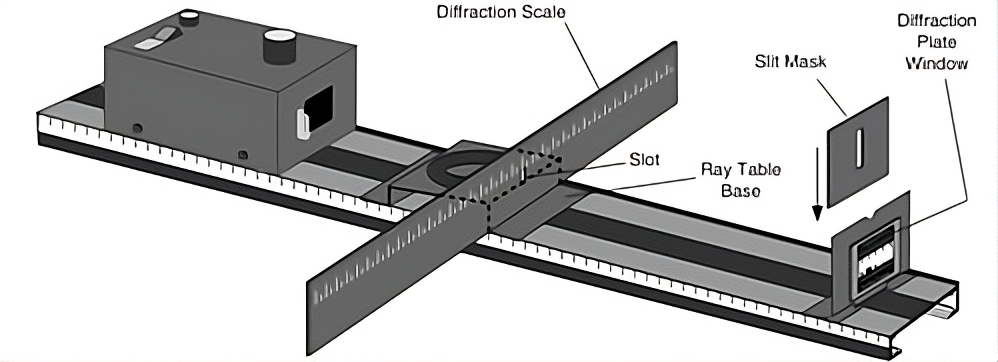
\includegraphics[width=0.8\linewidth]{figures/fig3.png}
    \caption{
    Montaje óptico utilizado en el laboratorio.
    Se observa la fuente de luz con la ranura y el filtro de color,
    seguida de la lente semicilíndrica convergente,
    la red de difracción (600 líneas/mm)
    y, a la derecha, la regla graduada usada como pantalla a una distancia $L \simeq \SI{0.205}{m}$.
    }
    \label{fig:montaje}
\end{figure}

En la práctica, la medición se realizó mirando a través de la red de difracción hacia la regla graduada. En esa vista aparecen simultáneamente el máximo central ($m=0$) y el primer máximo lateral ($m=1$) para un color dado. Definimos la distancia $x$ como la separación horizontal entre esas dos posiciones proyectadas sobre la misma escala, y $L$ como la distancia fija entre la red y la regla (ver Figura~\ref{fig:geometria_medicion}). Esta es exactamente la geometría que más tarde se usa en el análisis para calcular el ángulo $\theta$ y la longitud de onda $\lambda$.

    
\end{enumerate}

\subsection{Repetición del montaje}
Con el fin de evaluar la reproducibilidad, se repitió el ajuste óptico completo (posición relativa de la lente, red y regla). Llamaremos a estas dos sesiones \textit{primer montaje} y \textit{segundo montaje}. En ambos casos se midió $x$ para cada color y se usó el mismo valor de $L$.

\subsection{Tratamiento de datos}
Los datos ($x$, $L$, $a$) se procesaron en \texttt{Python} para obtener:
\begin{itemize}
    \item el ángulo $\theta = \arctan(x/L)$,
    \item la longitud de onda $\lambda$ usando \eqref{eq:lambda-experimental} con $m=1$,
    \item la incertidumbre de $\lambda$ por propagación de errores,
\end{itemize}

El código utilizado para realizar estos cálculos (carga de datos, conversión geométrica $x \mapsto \theta$, cálculo de $\lambda$ y propagación de errores) está disponible en línea; véase el script de análisis de datos en \href{https://udeconce-my.sharepoint.com/my?viewid=d66ef332%2Dcdd4%2D4011%2D840a%2D91d8ea92db3d&id=%2Fpersonal%2Fjrosas2022%5Fudec%5Fcl%2FDocuments%2FDatos%20adjuntos%2Flab%5Fcuantica%5F1%2Epy&parent=%2Fpersonal%2Fjrosas2022%5Fudec%5Fcl%2FDocuments%2FDatos%20adjuntos}{este enlace}.

En el tratamiento se asumieron incertidumbres instrumentales típicas
\[
    \delta x \approx 4\,\text{mm}, 
    \qquad
    \delta L \approx 2\,\text{mm},
\]
y se tomó $a \simeq 1{,}667\times10^{-6}\,\text{m}$ para la red (600 líneas/mm). La propagación de errores utilizada es coherente con derivadas parciales de \eqref{eq:lambda-experimental} respecto de $x$ y $L$.

Como ejemplo explícito, para la componente roja en el primer montaje se obtuvo
$x = 0{,}085\ \text{m}$ y $L = 0{,}205\ \text{m}$.
Primero calculamos el ángulo:
\[
\theta = \arctan\!\left(\frac{x}{L}\right)
= \arctan\!\left(\frac{0{,}085}{0{,}205}\right)
= 0{,}393\ \text{rad}.
\]

Con el paso de la red $a = 1{,}667\times10^{-6}\ \text{m}$ (600 líneas/mm) y usando sólo el primer orden ($m=1$), la ecuación experimental
\[
\lambda = a\,\frac{x}{\sqrt{x^{2}+L^{2}}}
\]
entrega
\begin{align*}
    \lambda
&= 1{,}667\times10^{-6}\ \text{m}\,
\frac{0{,}085\ \text{m}}{\sqrt{(0{,}085\ \text{m})^{2} + (0{,}205\ \text{m})^{2}}}\\
&= 6{,}38\times10^{-7}\ \text{m}\\
&= 638\ \text{nm}.
\end{align*}

Para la incertidumbre se usaron $\delta x \approx 0{,}004\ \text{m}$ y $\delta L \approx 0{,}002\ \text{m}$. Al aplicar la propagación de errores a $\lambda(x,L)$ se obtiene $\delta\lambda \approx 31\ \text{nm}$ para el rojo, valor que coincide con el tabulado en el Cuadro~\ref{tab:montaje1}.



\section{Resultados y análisis de datos.}

\subsection{Parámetros comunes}
En todas las mediciones se usó:
\begin{itemize}
    \item $L = (0{,}205 \pm 0{,}002)\,\text{m}$,
    \item $a = 1{,}667\times10^{-6}\,\text{m}$ (paso de la red),
    \item $m = 1$ (primer máximo de difracción),
    \item $\delta x \approx 0{,}004\,\text{m}$.
\end{itemize}

\subsection{Primer montaje}
En la Tabla~\ref{tab:montaje1} se resumen las mediciones del \textit{primer montaje}: desplazamiento $x$ para cada color, el ángulo asociado $\theta$, y la longitud de onda $\lambda$ obtenida. Se reporta además la incertidumbre típica $\delta\lambda$, que proviene de la propagación de errores en $x$ y $L$.

\begin{table*}
    \centering
    \caption{Resultados primer montaje ($m=1$). $\theta$ en radianes. $\lambda$ y $\delta\lambda$ en nm.}
    \label{tab:montaje1}
    \begin{tabular}{lcccccc}
        \toprule
        Color &
        $x$ [m] &
        $L$ [m] &
        $\theta$ [rad] &
        $\lambda$ [nm] &
        $\delta\lambda$ [nm] \\
        \midrule
        Rojo    & $0.085$ & $0.205$ & $0.393$ & $638$ & $31$ \\
        Verde   & $0.069$ & $0.205$ & $0.325$ & $532$ & $32$ \\
        Azul    & $0.061$ & $0.205$ & $0.289$ & $475$ & $33$ \\
        Morado  & $0.053$ & $0.205$ & $0.253$ & $417$ & $33$ \\
        Celeste & $0.063$ & $0.205$ & $0.298$ & $489$ & $33$ \\
        \bottomrule
    \end{tabular}
\end{table*}


Obsérvese que las longitudes de onda extraídas decrecen sistemáticamente al pasar de rojo a morado, lo que concuerda con el orden físico esperado del espectro visible (rojo $\sim$ longitudes de onda más largas; violeta/morado $\sim$ longitudes de onda más cortas).

\subsection{Segundo montaje}
Se repitió la medición tras reajustar el banco óptico. En el \textit{segundo montaje} se registraron nuevamente los distintos colores y además se identificaron componentes ``amarillo'' y ``naranja''. Los resultados se presentan en la Tabla~\ref{tab:montaje2}.

\begin{table*}
    \centering
    \caption{Resultados segundo montaje ($m=1$). $\theta$ en radianes. $\lambda$ y $\delta\lambda$ en nm.}
    \label{tab:montaje2}
    \begin{tabular}{lcccccc}
        \toprule
        Color &
        $x$ [m] &
        $L$ [m] &
        $\theta$ [rad] &
        $\lambda$ [nm] &
        $\delta\lambda$ [nm] \\
        \midrule
        Rojo     & $0.082$  & $0.205$ & $0.381$ & $620$ & $31$ \\
        Naranja  & $0.079$  & $0.205$ & $0.368$ & $600$ & $32$ \\
        Amarillo & $0.077$  & $0.205$ & $0.359$ & $586$ & $32$ \\
        Verde    & $0.069$  & $0.205$ & $0.325$ & $532$ & $32$ \\
        Celeste  & $0.0625$ & $0.205$ & $0.296$ & $486$ & $33$ \\
        Azul     & $0.060$  & $0.205$ & $0.285$ & $469$ & $33$ \\
        Morado   & $0.055$  & $0.205$ & $0.262$ & $432$ & $33$ \\
        \bottomrule
    \end{tabular}
\end{table*}

\subsection{Reproducibilidad y orden del espectro}
Comparando Tablas~\ref{tab:montaje1} y \ref{tab:montaje2} se ve que:
\begin{itemize}
    \item La luz roja se mantuvo en torno a $\sim 620\text{--}640$ nm.
    \item La luz verde se mantuvo en torno a $\sim 530$ nm.
    \item Las componentes azul/celeste/morado se ubicaron entre $\sim 430$ y $\sim 490$ nm.
\end{itemize}

Las diferencias entre el primer y el segundo montaje (por ejemplo, 638 nm vs 620 nm para el rojo) son comparables con la incertidumbre típica reportada ($\delta\lambda \sim 30$ nm). Esto indica que el método es consistente dentro del error de medición, dominado por la lectura de $x$ y la alineación geométrica.

% ======================================================
% 9. Discusión.
% ======================================================

\section{Discusión.}

\subsection{Consistencia física de los resultados}
El orden de magnitud de las longitudes de onda medidas coincide con lo esperado para la luz visible:
\begin{itemize}
    \item Rojo / naranja: $\lambda \sim (6{,}0 - 6{,}4)\times10^{-7}\,\text{m}$,
    \item Amarillo / verde: $\lambda \sim (5{,}3 - 5{,}9)\times10^{-7}\,\text{m}$,
    \item Celeste / azul / morado: $\lambda \sim (4{,}2 - 4{,}9)\times10^{-7}\,\text{m}$.
\end{itemize}
Este orden coincide con la clasificación cualitativa de colores observados.

Los valores típicos reportados en la literatura sitúan la luz roja en torno a $630\ \text{nm}$, la luz verde cerca de $530\ \text{nm}$ y la luz violeta por debajo de $450\ \text{nm}$ \cite{hecht_optics,young_freedman}. Nuestros resultados (por ejemplo, $638\ \text{nm}$ para el rojo y $417$--$432\ \text{nm}$ para el morado) coinciden con esos rangos dentro de la incertidumbre experimental de $\sim 30\ \text{nm}$, lo que valida el método de medición basado en la red de difracción.


\subsection{Reproducibilidad entre montajes}
Al repetir el montaje óptico (segundo montaje) se obtuvieron valores de $\lambda$ que, en promedio, no difieren más de unas decenas de nanómetros respecto del primer montaje. Dado que la propagación de errores con $\delta x \sim 4$ mm y $\delta L \sim 2$ mm entrega $\delta\lambda \sim 30$ nm, esas diferencias están dentro de la incertidumbre experimental.

Esto sugiere que la mayor fuente de error es geométrica:
\begin{itemize}
    \item Lectura del desplazamiento lateral $x$ sobre la regla observada ``a través'' de la red (paralaje).
    \item Alineación entre la red y el eje óptico: si la luz no incide perfectamente normal a la red, el máximo de primer orden puede desplazarse ligeramente.
    \item Determinación de $L$: aunque $L$ se mantuvo nominalmente en $0{,}205$ m, pequeños cambios de posición de la regla afectan el ángulo.
\end{itemize}

\subsection{Capacidad espectroscópica}
El hecho de que sea posible asociar valores de $\lambda$ distintos a rojo, naranja, amarillo, verde, etc., muestra que la red de difracción actúa como un espectrómetro elemental: diferentes longitudes de onda emergen en ángulos diferentes y por tanto aparecen en posiciones $x$ distintas sobre la regla.

En principio, si dos líneas espectrales son muy cercanas (por ejemplo, el doblete amarillo del sodio), sus máximos de difracción se verán muy próximos entre sí. Resolverlas como dos picos separados requiere:
\begin{itemize}
    \item una red con muchas ranuras iluminadas (alto poder de resolución),
    \item un montaje estable y bien alineado,
    \item baja incertidumbre en $x$.
\end{itemize}
En nuestro caso la incertidumbre típica de $\sim30$ nm es suficientemente grande como para que dos líneas demasiado cercanas pudieran aparecer como una sola franja ``engrosada''.

% ======================================================
% 10. Conclusiones.
% ======================================================

\section{Conclusiones.}

\begin{itemize}
    \item Se midió la difracción de la luz visible en una red de transmisión de 600 líneas/mm y se determinaron las longitudes de onda correspondientes a distintos colores del espectro visible usando la relación $a \sin\theta = m \lambda$ con $m=1$.
    \item Se obtuvieron valores típicos del orden de $\lambda \sim 4{,}2\times10^{-7}\,\text{m}$ (morado) hasta $\lambda \sim 6{,}4\times10^{-7}\,\text{m}$ (rojo), coherentes con el rango visible.
    \item La repetición del experimento con un segundo montaje arrojó resultados consistentes dentro de una incertidumbre típica de $\sim 30$ nm, lo que confirma la reproducibilidad cualitativa del procedimiento.
    \item El arreglo experimental funciona, en la práctica, como un espectrómetro simple: permite asignar longitudes de onda aproximadas a distintas componentes de color y sugiere cómo, con mejor control geométrico y menor error en $x$, podría incluso resolverse la presencia de líneas espectrales muy cercanas.
\end{itemize}

\begingroup
\raggedright
\printbibliography
\endgroup

\end{document}